\documentclass[12pt, a4papre]{article}
\usepackage[catalan]{babel}
\usepackage[unicode]{hyperref}
\usepackage{amsmath}
\usepackage{amssymb}
\usepackage{amsthm}
\usepackage{xifthen}
\usepackage{siunitx}
\usepackage{xcolor}
\usepackage{float}
\usepackage{listings}
\usepackage{setspace}
\usepackage{graphicx}
\usepackage{tikz,lipsum,lmodern}
\usepackage[most]{tcolorbox}
\usepackage{circuitikz}
\usepackage{indentfirst}
\usepackage{verbatimbox}
\definecolor{mygreen}{RGB}{28,172,0} % color values Red, Green, Blue
\definecolor{mylilas}{RGB}{170,55,241}

\graphicspath{ {./images/} }


\newcommand{\norm}[1]{\lvert #1 \rvert}

\hypersetup{
    colorlinks = true,
    linkcolor = blue
}

\author{Daniel Vilardell\\
	   Igor Yuziv}
\title{Memoria practica 1 DGD}
\date{17-10-2020}

\begin{document}
	\maketitle
	Aquesta primera practica es divideix en dos parts, la part a i la part b. La primera part es basa en aprendre com funciona el programa Quartus II a partir de fer un multiplexor  2:1 per a bussos de 4 bits i verificar el seu funcionament sobre la placa DE2. En la segona part, aplicant el coneixement adquirit en la primera, construim una calculadora que permet multiplicar dos nombres de 4 bits en CA2.
	
	En aquesta memoria explicarem detalladament la construccio de cada component i com s'usa per a assolir els objectius proposats.

	\newpage
	\section{Primera part}
	\textbf{\large{Multiplexor 2:1}}
	
	Crearem un multiplexor 2:1 amb el diagrama de blocs:
	\begin{figure}[H]
		\begin{center}
		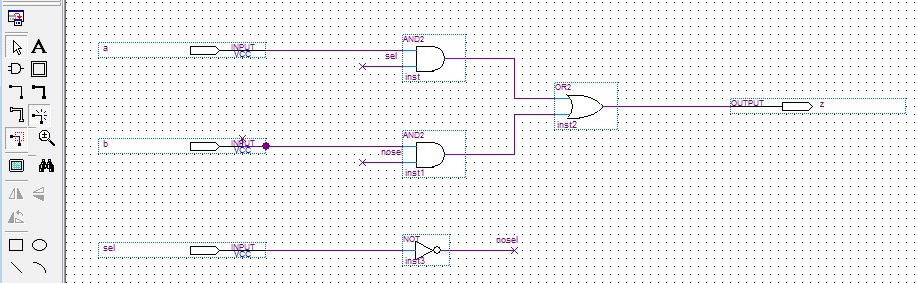
\includegraphics[width=150mm]{multiplexor2_1.jpeg}
		\end{center}
	\end{figure}
	
	Una vegada descrit el circuit anirem a sintetitzar-lo de forma que pugui ser
simulat, validat i gravat en la FPGA. Primer hem de seleccionar la nostra descripció com a entitat de nivell més alt, seguidament fer servir el Compilador.
		\begin{figure}[H]
		\begin{center}
		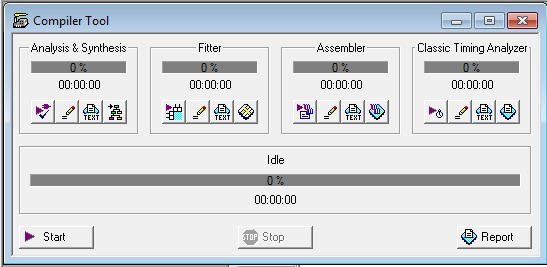
\includegraphics[width=100mm]{simulador.jpeg}
		\end{center}
	\end{figure}
	\begin{figure}[H]
		\begin{center}
		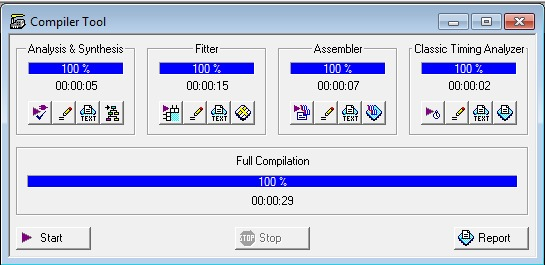
\includegraphics[width=100mm]{simuladorfet.jpeg}
		\end{center}
	\end{figure}
	
	Un cop hem sintetitzat el circuit anirem a simularlo amb el "Debugging File" que serà "Vector Wave File"
	
	\begin{figure}[H]
		\begin{center}
		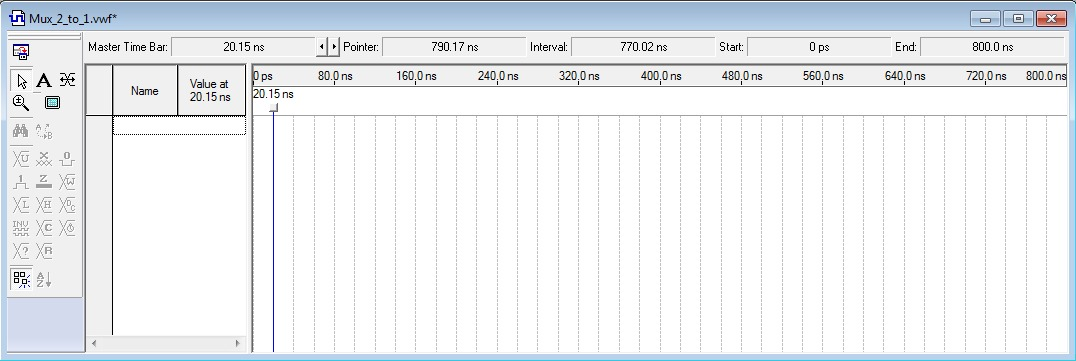
\includegraphics[width=140mm]{waveform.jpeg}
		\end{center}
	\end{figure}
	
	Un cop aqui tindrem que seleccionar els nodes que volem que apareixin a la simulació.
	\begin{figure}[H]
		\begin{center}
		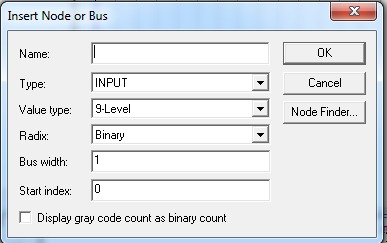
\includegraphics[width=60mm]{Insertnode.jpeg}
		\end{center}
	\end{figure}
	
	Donarem el boto de  Node Finder i seleccionarem els nodes que ens interesa per simular.
	
		\begin{figure}[H]
		\begin{center}
		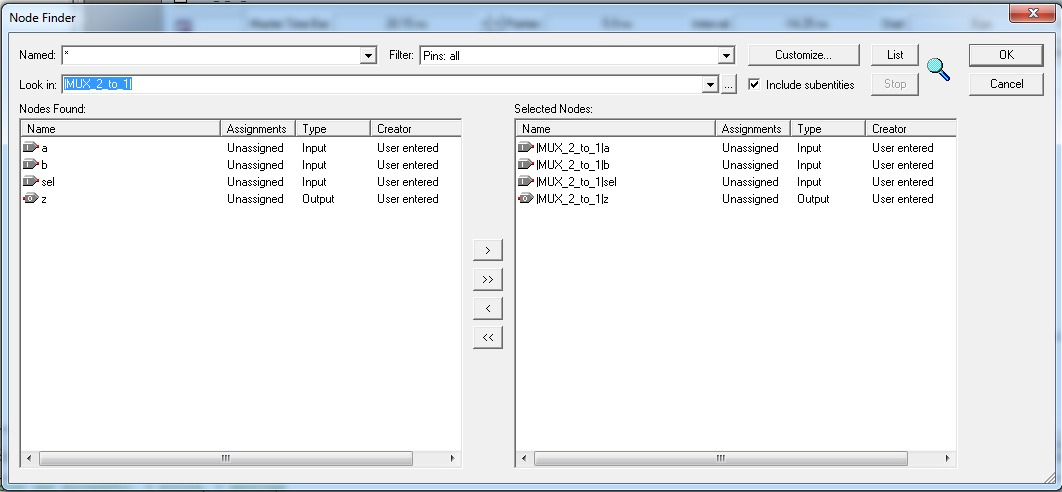
\includegraphics[width=150mm]{nodes.jpeg}
		\end{center}
	\end{figure}
	
	Una vegada que tenim els nodes seleccionats procedirem a canviar els valors dels nodes per poder fer la simulació.
	
		\begin{figure}[H]
		\begin{center}
		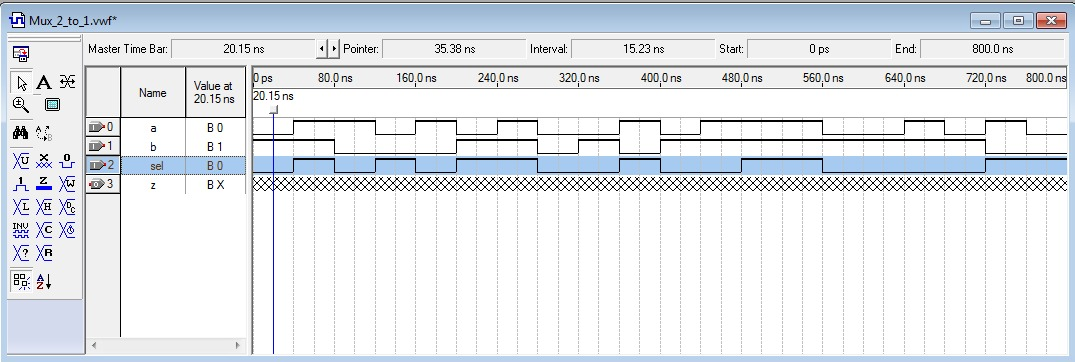
\includegraphics[width=150mm]{simulacioambvalors.jpeg}
		\end{center}
	\end{figure}
	
	Finalment farem la simulació i mirarem si ens done el resultat esperat. Per fer la simulació farem servir el "Simulator Tool".
	\begin{figure}[H]
		\begin{center}
		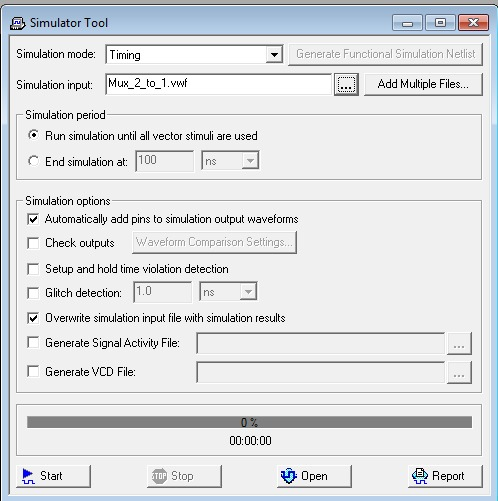
\includegraphics[width=120mm]{finestrasimulacio.jpeg}
		\end{center}
	\end{figure}
	
	Com es pot veure aqui la simulació ja esta feta i el circuit es comporta com esperavem.
	\begin{figure}[H]
		\begin{center}
		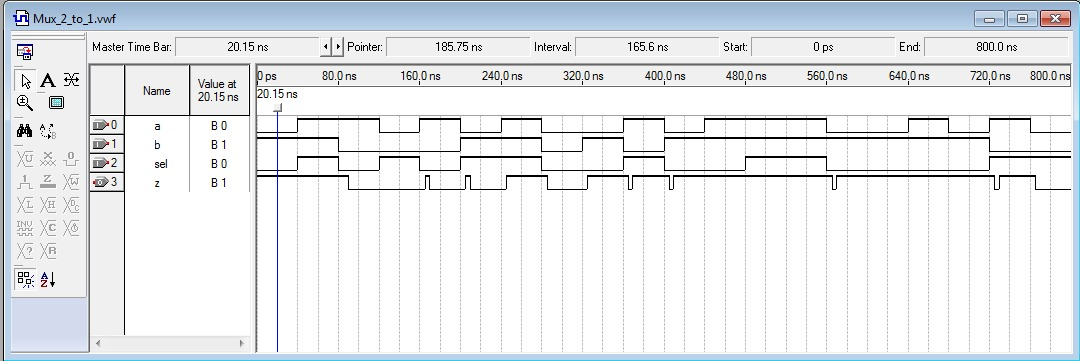
\includegraphics[width=150mm]{simulaciofeta.jpeg}
		\end{center}
	\end{figure}
	
	\textbf{\large{Multiplexor 2:1 per busos de 4 bits}}
	
	Per fer el Multiplexor primer tindrem que crear un nou bloc amb el Multiplexor 2:1.
	
	\begin{figure}[H]
		\begin{center}
		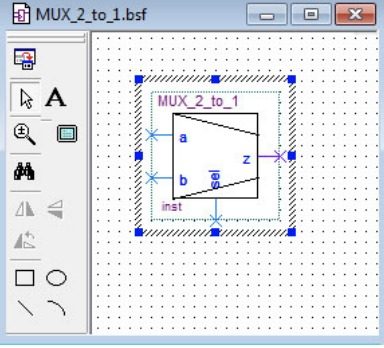
\includegraphics[width=80mm]{blocmultiplexor.jpeg}
		\end{center}
	\end{figure}
		
	Un cop tenim el bloc del multiplexor, procedirem a fer el circuit del Multiplexor 2:1 per busos de 4 bits
		\begin{figure}[H]
		\begin{center}
		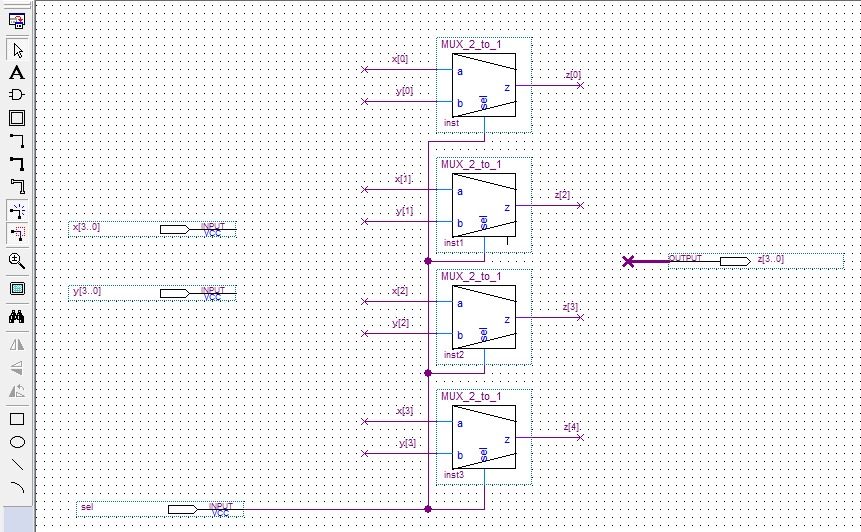
\includegraphics[width=150mm]{mult4bits.jpeg}
		\end{center}
	\end{figure}
	
		Un cop creat el bloc compilarem i simularem per comprobar el correcte funcionament i crearem un nou bloc per poder utilitzarlo quan el nesesitarem.
	
	\begin{figure}[H]
		\begin{center}
		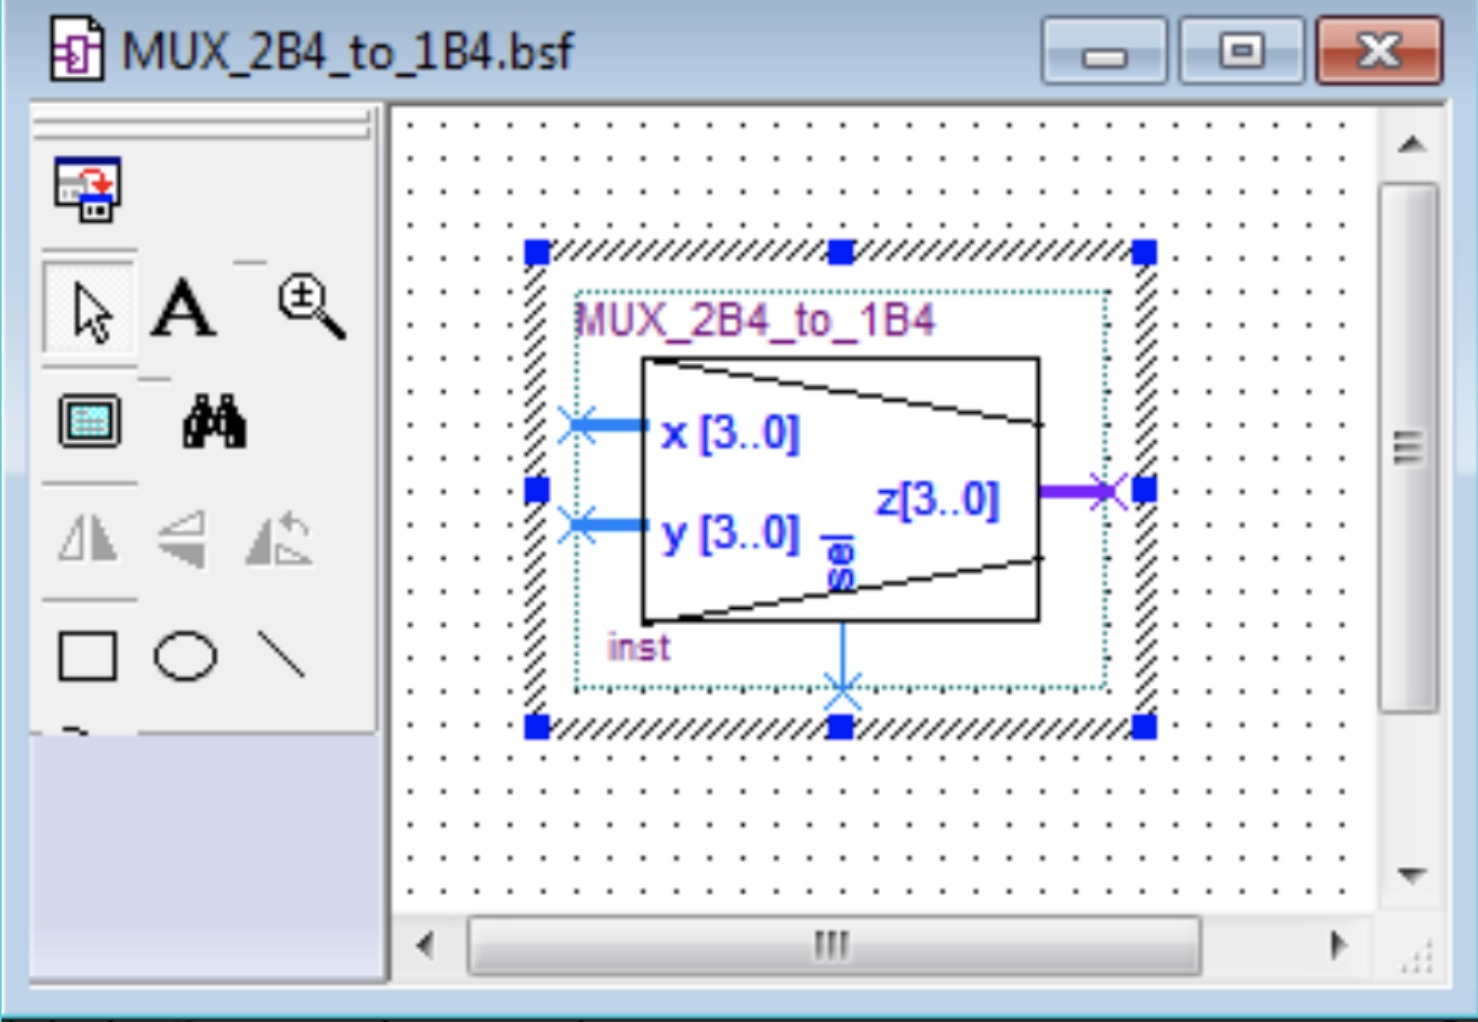
\includegraphics[width=80mm]{blocnoumult.jpeg}
		\end{center}
	\end{figure}
	
	\textbf{\large{Convertidors de BCD a set segments}}
	
	Per poder utilitzar els convertidors de BCD els importarem al projecte i muntarem el circuit, com es mostra a la següent figura.
	
	\begin{figure}[H]
		\begin{center}
		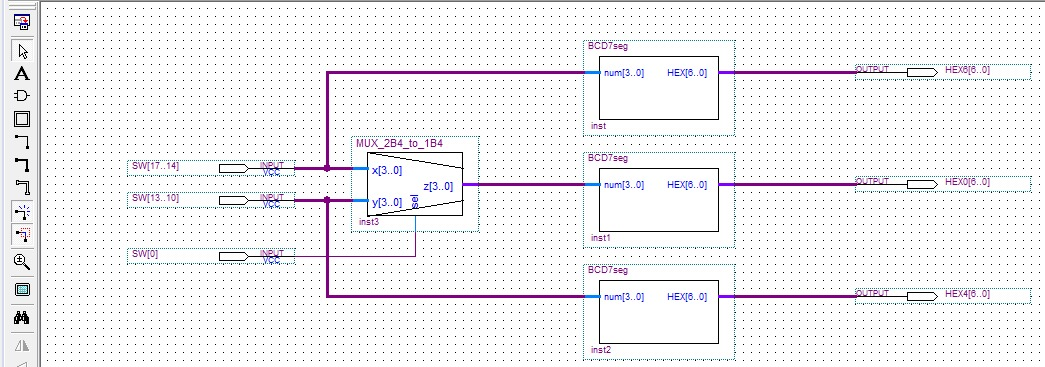
\includegraphics[width=150mm]{bcd7.jpeg}
		\end{center}
	\end{figure}
	
	Un cop tenim el circuit complet dissenyat, hem de convertir-lo en el nivell de jerarquia més
alt amb "Set as Top-Level Entity".\\

	
	\textbf{\large{Asignació de pins}}	
	
	Per poder simular el nostre circuit a la placa FPGA tindrem que importar l'asignació de pins desde el document excel que ens proporcionen, associa cada pin de la FPGA amb el nom del senyal del component de la placa on està connectat. 
	\begin{figure}[H]
		\begin{center}
		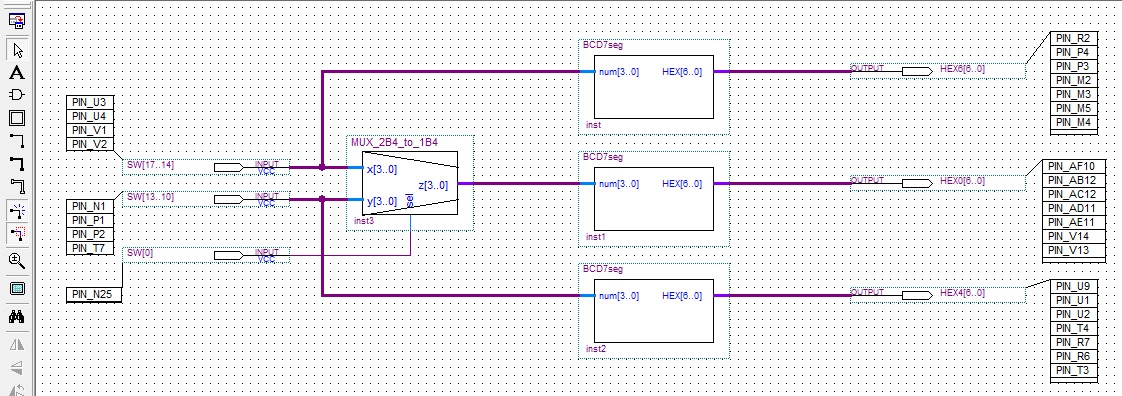
\includegraphics[width=150mm]{bcd7segasign.jpeg}
		\end{center}
	\end{figure}
	
	Finalment farem la simulació del disseny complet per comprobar el seu funcionament i poder enviarlo a la placa FPGA.
	\begin{figure}[H]
		\begin{center}
		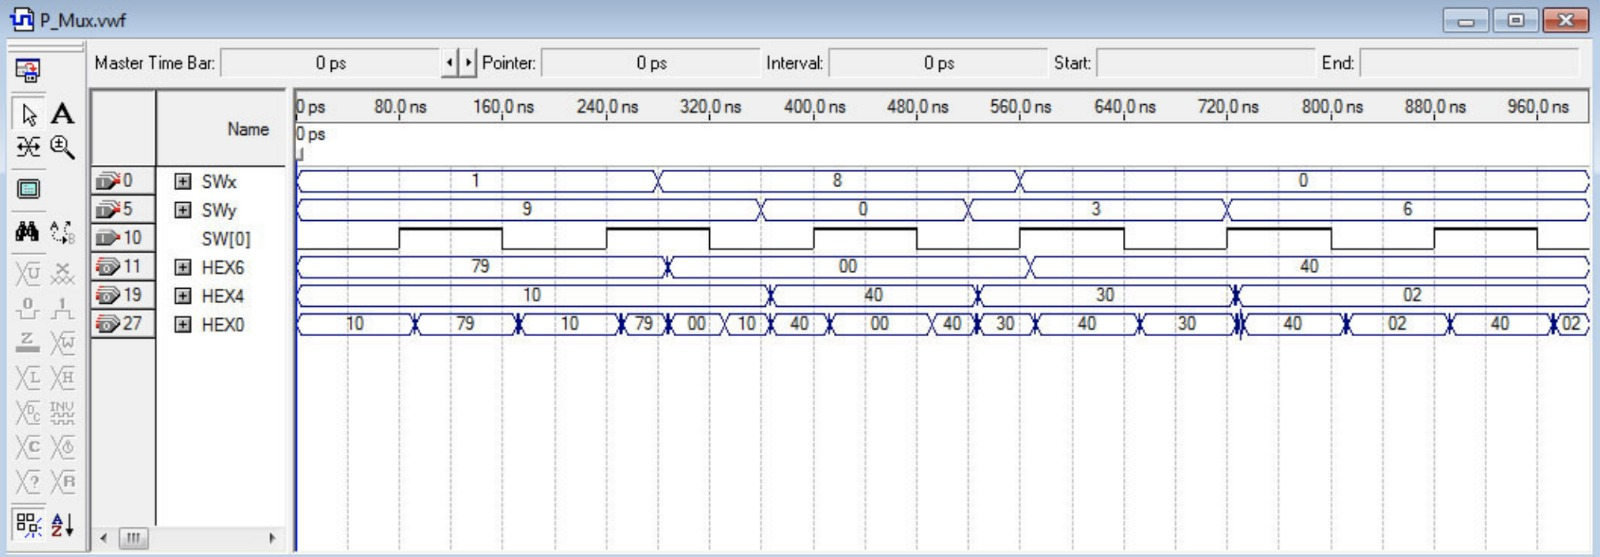
\includegraphics[width=150mm]{simulfinal.jpeg}
		\end{center}
	\end{figure}
	
	
	\textbf{\large{Validació del disseny sobre la placa DE2}}	
	
	Engegarem la font d’alimentació i posarem la tensió de sortida a uns 8.5V. Connectarem el cable
	USB a l’entrada USB-Blaster de la placa DE2 i a un port USB del PC.  Clicarem l’interruptor vermell de la placa.
	Un cop encesa  procedirem a programar la placa .
	
	\begin{figure}[H]
		\begin{center}
		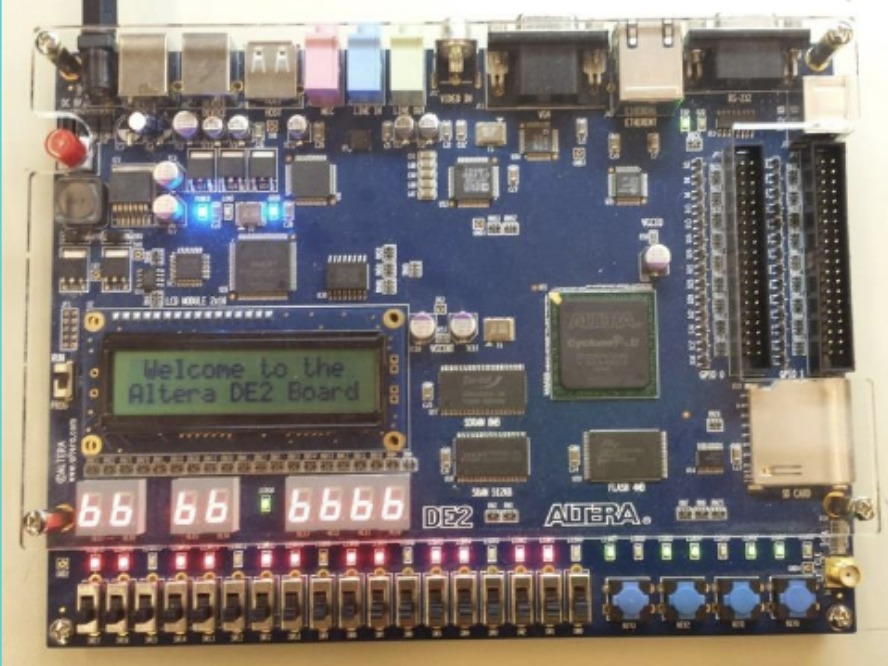
\includegraphics[width=120mm]{placa.jpeg}
		\end{center}
	\end{figure}
	
	
	Per poder programar la placa anirem a "tools - Programmer".
	\begin{figure}[H]
		\begin{center}
		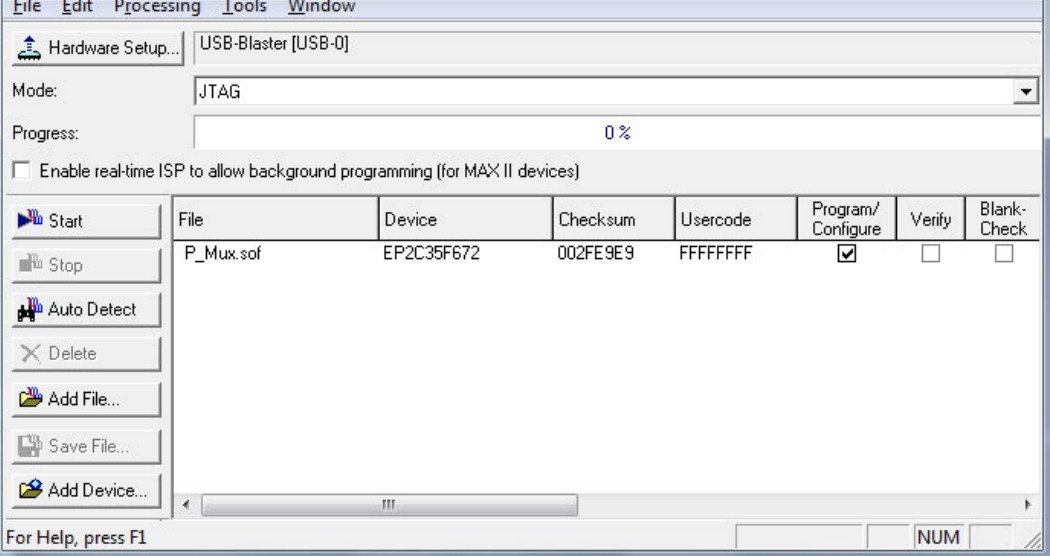
\includegraphics[width=150mm]{programacioplaca1.jpeg}
		\end{center}
	\end{figure}
	
	\newpage
	\section{Segona part}
	\textbf{\large{Convertidor de CA2 de 4 a 8 bits}}
	
	Aquest component es ben simple i s'usara per a poder fer el producte de dos nombres en CA2 ja que el resultat de la multiplicació és sempre un nombre de 8 bits. El que fa es agafar el bit de mes pes de la entrada i el repeteix als bits de mes pes seguents. La rao per la que funciona aquesta idea ja està vista al previ
	
	\begin{figure}[H]
		\begin{center}
		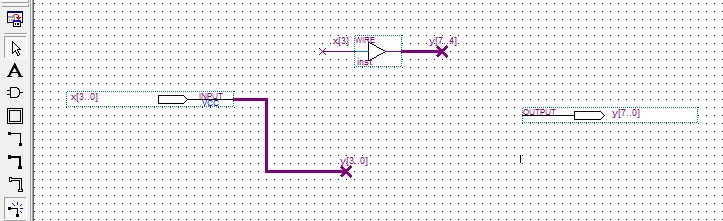
\includegraphics[width=150mm]{CA2_4_a_8.jpeg}
		\end{center}
	\end{figure}
	\begin{figure}[H]
		\begin{center}
		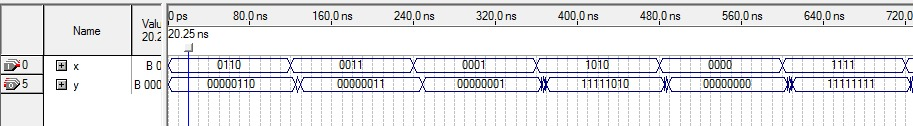
\includegraphics[width=150mm]{CA2_4A8simul.jpeg}
		\end{center}
	\end{figure}
	
	\textbf{\large{Multiplicador 8x1}}
	
	Aquest component multiplica un nombre de 8 bits per  un nombre de 1 bit. Per tant la sortida sera el nombre de 8 bits entrat si l'altre nombre es 1, i 0 altrament.
	
	\begin{figure}[H]
		\begin{center}
		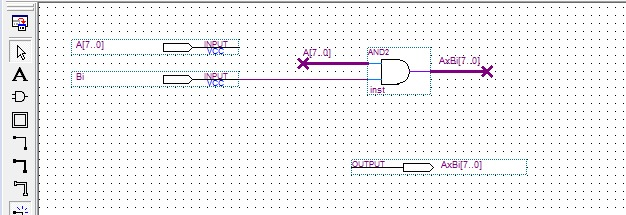
\includegraphics[width=150mm]{MULT8x1.jpeg}
		\end{center}
	\end{figure}
	
	\begin{center}
	
	\begin{figure}[H]
		\begin{center}
		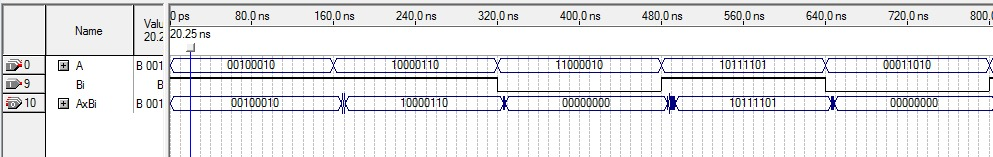
\includegraphics[width=150mm]{MULT8x1simul.jpeg}
		\end{center}
	\end{figure}
	
	\end{center}
	
	\textbf{\large{Multiplicador i sumador}}
	
	Aquest component te la funcio de multiplicar un nombre de 8 bits per un de 1 usant el component mencionat anteriorment per després sumar el resultat amb un altre nombre de 8 bits que ve a l'entrada. Això es fara servir per a fer la multiplicacio classica que es basa en multiplicar un per un els bits del nombre de baix i sumar amb els anteriors sempre treient el bit de menys pes. Es per aixo que les sortides del component son per una banda el bit de menys pes que s'usara per a posar al resultat, i per altra els 7 bits de mes pes resultants de la suma. 
	
	\begin{center}
	\begin{figure}[H]
		\begin{center}
		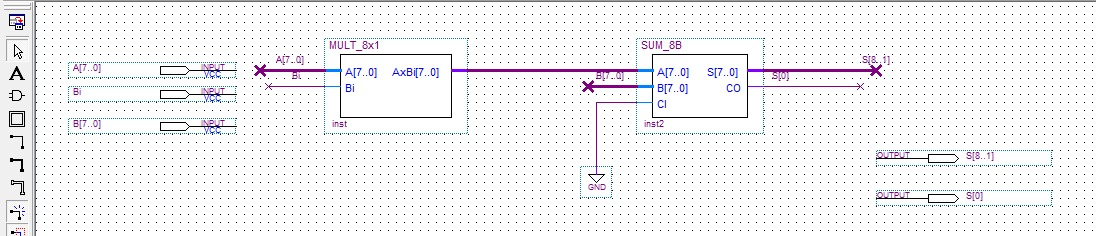
\includegraphics[width=150mm]{MULT_+SUM.jpeg}
		\end{center}
	\end{figure}
	
	\end{center}
	
	
	\textbf{\large{Multiplicador binari de 8 bits}}
	
	Aquest component multiplica dos nombres de 8 bits a partir de posar en serie els muliplicadors i sumadors comentats abans. La entrada son dos nombres de 8 bits, i a cada entrada dels 8 components en serie s'hi posarà el nombre de dalt, es a dir A[7..0], el bit que toqui del nombre de baix, B[i] i finalment se li entrarà la suma de les anteriors multiplicacions extreient el bit de menys pes. Aquest bit de menys pes anirà al nombre de 16 bits que hi ha a la sortida. Finalment quan s'arriba al últim component s'introdueix tota la sortida (la suma i el bit de menys pes) a la sortida general del component.
	
	\begin{center}
	\begin{figure}[H]
		\begin{center}
		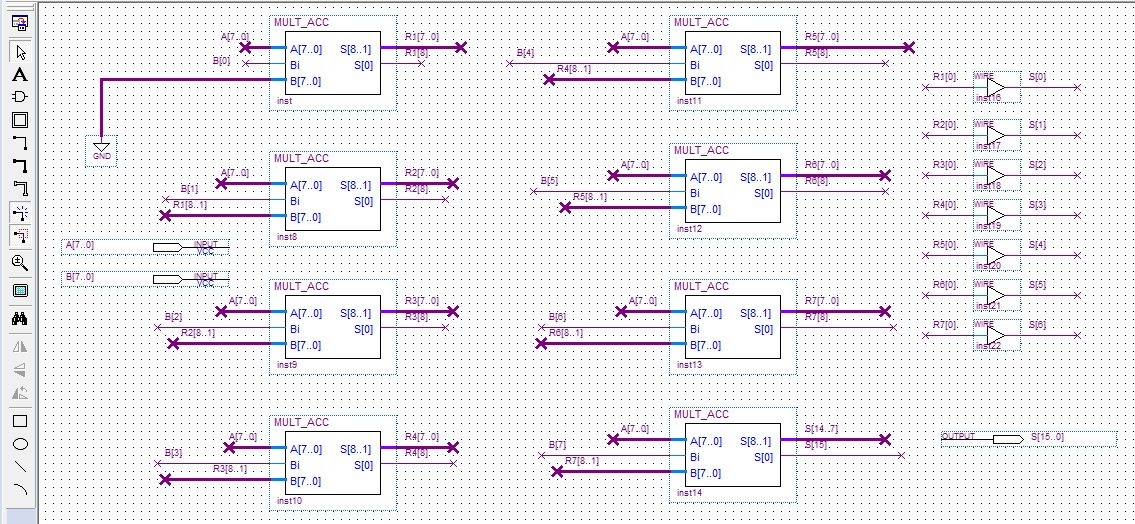
\includegraphics[width=150mm]{multbin8bits.jpeg}
		\end{center}
	\end{figure}
	
	\end{center}
	
	\begin{center}
	\begin{figure}[H]
		\begin{center}
		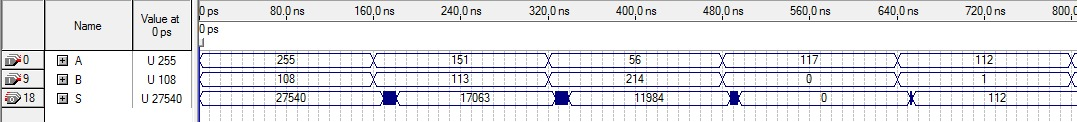
\includegraphics[width=150mm]{multbin8bitssimul.jpeg}
		\end{center}
	\end{figure}
	
	\end{center}
	
	
	
	
	\textbf{\large{Multiplicador CA2 de 4 bits}}
	
	Aquest component multiplica dos nombres en CA2 de 4 bits. Per a fer això primer els transforma a CA2 de 8 bits amb el primer component mencionat, per a despres introduirlo al multiplicador binari de 8 bits. Tot i que la sortida es de 16 bits, nomes ens interessen els 8 bits de menys pes ja que al multiplicar dos nombres de 4 bits, el resultat maxim tindrà 8 bits.
	
	
	\begin{center}
	\begin{figure}[H]
		\begin{center}
		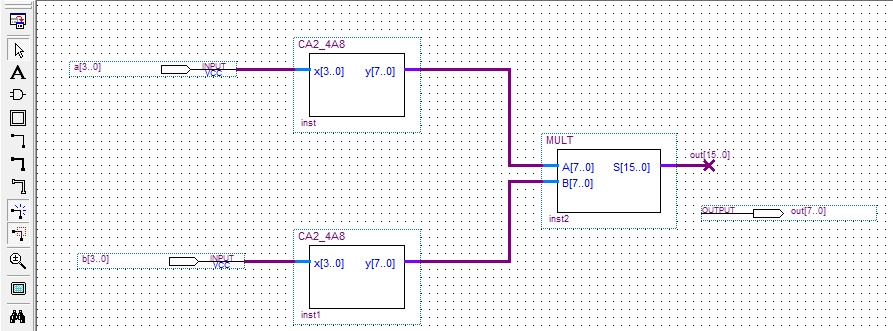
\includegraphics[width=150mm]{multCA2_4B.jpeg}
		\end{center}
	\end{figure}
	
	\end{center}
	\begin{center}
	\begin{figure}[H]
		\begin{center}
		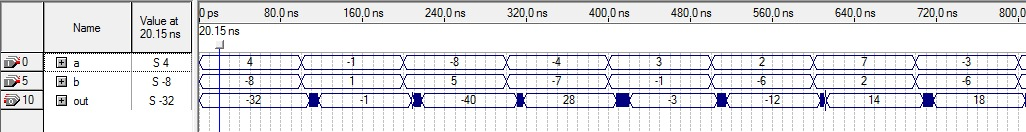
\includegraphics[width=150mm]{multCA2_4Bsimul.jpeg}
		\end{center}
	\end{figure}
	
	\end{center}
	
	
	\textbf{\large{Adaptador de signe}}
	
	Aquest component te la finalitat de veure si el valor es negatiu o positiu i en el cas de que sigui negatiu, encen el segment de la placa corresponent per a que pugui ser visualitzat.
	
	\begin{center}
	\begin{figure}[H]
		\begin{center}
		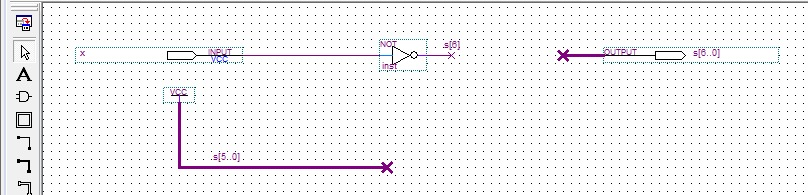
\includegraphics[width=150mm]{adaptSigne.jpeg}
		\end{center}
	\end{figure}
	
	\end{center}
	
	\textbf{\large{Convertidor CA2 de 4 bits al seu modul}}
	
	Aquest component es el que ens permetrà extreure el modul de un nombre en CA2 de 4 bits per tal de representarlo a la placa.
	
	\begin{center}
	\begin{figure}[H]
		\begin{center}
		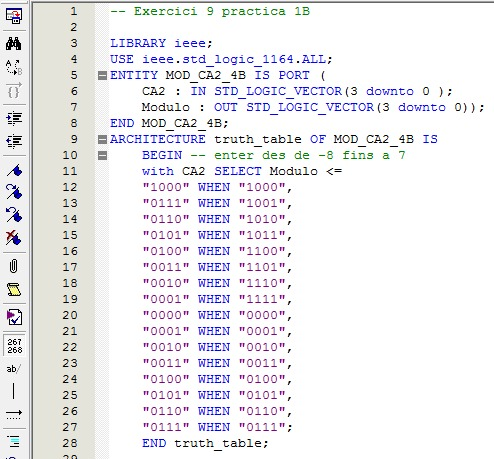
\includegraphics[width=100mm]{ConvCA2_4aMOD.jpeg}
		\end{center}
	\end{figure}
	
	\end{center}
	
	\textbf{\large{Multiplicador final per a visualització}}
	
	Aquesta multiplicació final te tres branques, una per a la visualització del primer nombre entrat, una per a la visualització del segon i finalment una per a visualitzar el resultat. La entrada sera de dos nombres de 4 bits als que assignarem pins de la placa. 
	
	La primera branca i la segona funcionen igual així que només explicarem una d'elles. 
	\begin{enumerate}
	\item Quan s'entra un nombre en CA2 de quatre bits, primer determinem el signe amb el adaptador de signe. Aquesta sortida ja va directe a la placa i mostra el signe.
	\item Després de determinar el signe es converteix el nombre en CA2 al seu modul.
	\item Quan ja tenim el modul l'introduim a un component facilitat per la assignatura que converteix nombres binaris de 4 bits a BCD de 7 segments. Aquesta sortida també va directe a la placa i mostra el nombre.
	\end{enumerate}
	
	La tercera i ultima branca funciona de la següent manera:
	\begin{enumerate}
	\item Primer s'introdueixen els dos nombres al multiplicador CA2 de 4 bits, el qual dona el seu producte en CA2.
	\item S'extreu el signe a partir del bit de mes pes i es mostra a la placa usant el adaptador de signe.
	\item La sortida del producte s'introdueix dins del component facilitat també per la assignatura que et dona el BCD de un nombre de 8 bits.
	\item Els primers 4 bits seran el primer nombre de la sortida, així doncs aquest nombre es passa a BCD de 7 segments i es mostra a la placa.
	\item Finalment es fa el mateix pels 4 ultims bits, els de menys pes, i es mostra a la placa.
	\end{enumerate}
	
	\begin{center}
	\begin{figure}[H]
		\begin{center}
		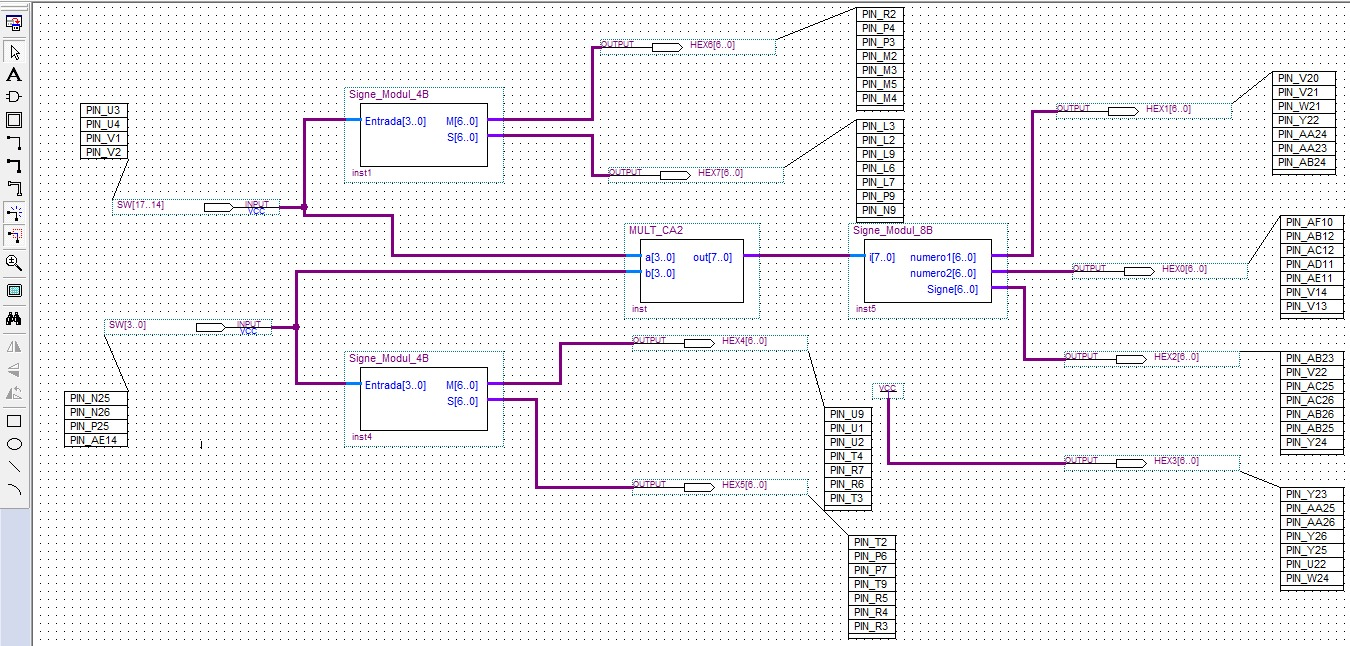
\includegraphics[width=150mm]{multFinal.jpeg}
		\end{center}
	\end{figure}
	
	\end{center}
	
	\newpage
	\section{Tercera part(extra)}
	
	Un cop implementada la calculadora que permet fer el producte de dos nombres en CA2, ara sens proposa que montem un component que a partir de tres entrades, A B i selop tregui la sortida seguent:
	
	\begin{itemize}
	\item $A\cdot B$ si selop $=00$
	\item $A^2$ si selop $=01$
	\item $B^2$ si selop $=10$
	\item$2^A\cdot2^B$ si selop $=11$
	\end{itemize}
	
	Cal tenir en compte en primer lloc que la sortida es de 8 bits, i per tant la sortida $2^A\cdot2^B$ no podra mostrar totes les sortides possibles. Tenint en compte que com la sortida es en CA2, nomes disposem de 7 bits i per tant nomes podrem representar totes aquelles sortides tals que $A+B \leqslant 7$. A mes a mes, com que nomes podem representar nombres enters, la suma de $A+B \geqslant 0$. 
	
	Vist aixo ara cal pensar com farem el diseny del cirquit. En el nostre cas primer escollirem quins dos nombres multiplicar, es a dir, si selop es 00, escollirem per una banda $A$ i per altra banda $B$. Si selop es 01 escollirem $A$ i $A$, si selop es 10 escollirem $B$ i $B$. Finalment si selop es 11, com que no ens importa el resultat del producte ja que la sortida vindra d'un altre component que fara el calcul $2^A\cdot2^B$, multiplicarem $0\cdot 0$.
	
	Per a fer la seleccio primer fem un multiplexor 2x1, que usarem per a construir altres components mes grans.
	
	\textbf{\large{Multiplexor 2x1}}
	
	Aquest component es ben senzill, te tres entrades de 1 bit: $A$, $B$, i $X$. Si $X=0$ la sortida sera $A$, si $X=1$ la sortida sera $B$.
	
	\begin{center}
		FOTO COMPONENT
		
		FOTO SIMULACIO
	\end{center}
	
	\textbf{\large{Multiplexor 4x1}}
	
	Aquest es igual de senzill que l'anterior. Se li donen sis entrades, quatre de informació i dos de seleccio. En funcio de les de seleccio s'extreu una  o una altre de les de informacio per la sortida.
	
	\begin{center}
		FOTO COMPONENT
		
		FOTO SIMULACIO
	\end{center}
	
	\textbf{\large{Selector mult}}
	
	Amb el multiplexor 4x1 ja en vam tenir prou per a disenyar el component que s'encarregaria de seleccionar i retornar els dos nombres que s'estan multiplicant. La entrada del component son dos nombres de 4 bits A i B, i selop, de dos bits. 
	
	Per a construir el primer nombre de la sortida usarem els multiplexors, a les entrades els hi posarem $A$[i], $A$[i], $B$[i] i 0 on i es cada xifre. La sortida la dirigirem al digit $i$ del vector de 4 bits de la sortida. A la entrada de seleccio hi posarem selop. Per tant si selop és $00$ el primer component que treura serà $A$, si es $01$ treura $A$, si es $10$ treurà $B$ i 0 si es 11, per la rao comentada abans.
	
	La segona sortida sera construida de la mateixa forma pero a la entrada del multiplexor se li posara $B$[i], $A$[i], $B$[i] i 0.
	
	\begin{center}
		FOTO COMPONENT
		
		FOTO SIMULACIO
	\end{center}
	
	\textbf{\large{Elevador}}
	
	Aquest component te la funcio de donades dos entrades $A$ i $B$ si $A + B < 7$ o $A + B  < 0$ treure dos sortides, una que sigui 0 i l'altre serà 1, aquesta segona sera la que permetrà que el led s'ilumini. Si la suma està dins dels valors permesos, la primera sortida serà $2^A\cdot2^B$ i la segona sortida sera 0, ja que en aquest cas el bit no s'haurà d'iluminar.
	
	Aquest component ha estat fet amb vhdl per comoditat.
	
	\begin{center}
		FOTO COMPONENT
		
		FOTO SIMULACIO
	\end{center}
	
	\textbf{\large{Multiplexor 2x1 per entrades de 4 bits}}
	
	Aquest component ens servira per a simplificar el diseny final de la calculadora. Fa el seguent: Donats dos nombres de 4 bits $A$ i $B$ i un nombre de seleccio de 2 bits selop, si selop es 00, 01 o 10 la sortida sera $A$, si selop es 11 la sortida es $B$.
	
	\begin{center}
		FOTO COMPONENT
	\end{center}
	
	\textbf{\large{Calculadora}}
	
	Aquest component serà el que ens fara el calcul. Donades 3 entrades, $A$, $B$ i selop primer es passaran les tres entrades per el component selector mult, que ens retornara quins dos nombres multiplicar. Aquestes dos sortides amb la ajuda de CA2 4 - 8 bits passarem les 2 sortides de 4 a 8 bits en CA2. Aquestes sortides s'introduiran al multiplicador que ens retornarà el seu producte en CA2. 
	
	Per altra banda, introduirem $A$ i $B$ al elevador del que hi haurà dos sortides. La segona d'elles ens informarà si s'ha de iluminar el led en el cas de que selop fos 11. Per a veure si es 11 o no usarem un multiplexor de 1 bit on les tres primeres entrades estaran conectades a terra i la última entrada estarà conectada a la sortida del bit d'error del elevador. Les entrades de seleccio seran selop. La sortida del multiplexor ens dirà si s'haurà d'iluminar el bit d'error o no.
	
	Ara usarem un multiplexor 2x1 per entrades de 4 bits a on se li posarà la sortida del multiplicador a la primera entrada, la sortida del elevador a la segona entrada i selop a les entrades de selecció. La sortida d'aquest component sera el valor buscat.
	
	\begin{center}
		FOTO COMPONENT
		
		FOTO SIMULACIO
	\end{center}
	
	\textbf{\large{Simulador calculadora}}
	
	Aquest component es el que enviarem a la placa, per tant te l'objectiu de llegir les entrades dels pins i mostrar els resultats per pantalla.
	
	Consta de tres entrades, $A$ $B$ i selop. De la matexa manera que en la segona part de la practica es mostraran les entrades $A$ i $B$ a la placa. 
	
	Les entrades s'introduiran dins del component calculadora. Aquest ens extreura el calcul per una banda, que despres de passarlo per el conversor de nombre de 8 bits en CA2 a BCD de 7 segments l'enviarem a la sortida per a que sigui mostrat a la placa. Per altra banda ens extreura si ca encendre el bit d'error en el calcul o no, que enviarem també al la placa directament.
	
	\begin{center}
		FOTO COMPONENT
	\end{center}
	
	
	
\end{document}